\subsection{Robot bevægelse}
% Bevægelses mønster
For at robotter kan opnå bevægelse anvendes der led ligesom ved mennesker og dyr, til at udføre fremad og bagudrettet bevægelser, samt rotation om led. Gennem en kombination af flere led og led typer, opnår robotter forskellige bevægeles muligheder. 

% Joint(led) typer
Der er fire typer af led som primært bruges og de kan opdeles i en lineær gruppe og rotations gruppe. To af ledtyperne er lineære led og glidende led, som muliggøre bevægelse på en akse. De to andre led er rotationsled og kugleled. Rotationsled muliggøre rotation om et punkt i et plan og udfører derved bevægelser på to akser, ved at rotere om en tredje akse, se figur \ref{fig:rotation i planet}. Kugleled muliggøre bevægelse på tre separate akser, hvilket betyder der er tale om 3D bevægelser. Kugleled har derigennem også muligheden for at fungere som rotationsled, ved ikke at bevæge sig på den tredje akse \parencite{Niku2020IntroductionApplications}. Sammensætninger af led typer kan ses på \ref{fig: Sammensætniger af led}.
\begin{figure} [H]
    \centering
    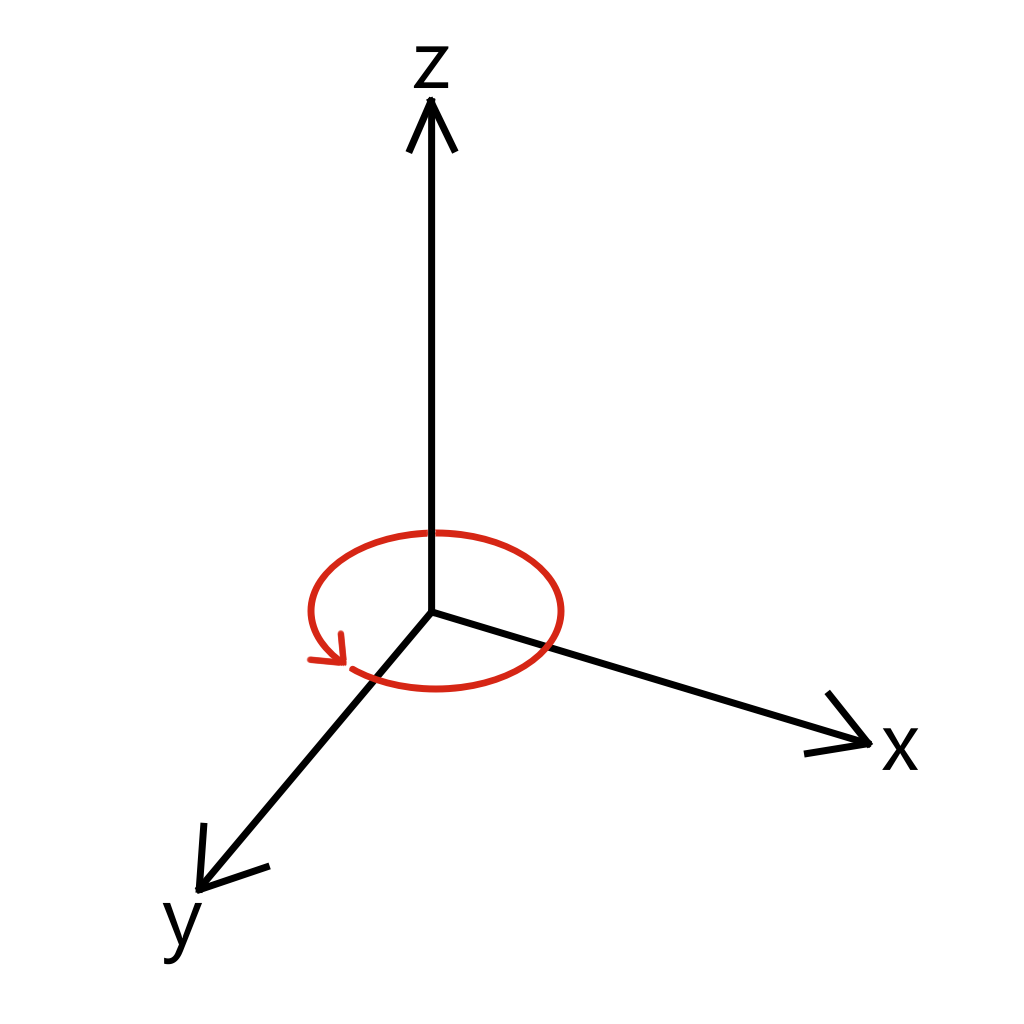
\includegraphics[width=0.4\linewidth]{Sections/2 Problemanalyse/Media/Rotation i planet.png}
    \caption{Illustration af rotation i et xy-plan, omkring z-aksen.}
    \label{fig:rotation i planet}
\end{figure}
% Degree of freedom(on/off)
De forskellige ledtyper giver forskellige mængder af frihedsgrader, hvilket er en angivelse af bevægelsesmulighederne for en robot. Desto større mængde af frihedsgrader, desto mere komplekse bevægelser kan en robot udføre. Dette betyder også at mængden af bevægelsesudregninger øges i takt med at frihedsgraden stiger. Hvert led har en frihedsgrads værdi som angiver hvor mange akser leddet kan bevæge sig på eller rotere omkring. Ved tilfælde hvor bevægelsen kun kan være binære, som ved en skinne der er skubbet helt ud eller slet ikke skubbet ud, angives der en halv frihedsgrad. Den totale sum af alle leds frihedsgrader er en robots frihedsgrads værdi. 

\begin{figure} [H]
    \centering
    \includegraphics[width=0.8\linewidth]{Sections/2 Problemanalyse/Media/Sammensætninger af led typer.png}
    \caption{Eksempler på sammensætninger af led, der giver anledning til forskellige bevægelses mønster og muligheder. Billedet er fra\parencite{Niku2020IntroductionApplications}}
    \label{fig: Sammensætniger af led}
\end{figure}

% Kalibering(waypoints)
For at robotter har en forståelse af hvor de er og hvor en bevægelse vil placere dem, anvendes der to forskellige tilgange. Den første gør brug af sensor observation, til gennem inputs at klargøre hvordan verden ser ud, som nævnt i afsnit \textit{2.1}. Den anden tilgang gør brug af man forklarer robotten hvordan verden omkring den ser ud. Dette gøres ved software repræsentation, manuel kalibrering eller en kombination. Manuel kalibrering er en udbredt metode, som gør brug af man fastlægger waypoints, hvilket er et sæt punkter robotten bruger som reference. Waypoints fastlægges ved at manuelt styre robotten til de ønsket reference punkter og derved fastlægge dem.

De to tilgange anvendes sjældent hver for sig, men vil derimod ofte blive brugt i kombination til at løse forskellige problemstillinger en robot vil stå med. Eksempelvis produktions- og pakkeriindustrirobotter gør brug af forklarings metoden til at udføre deres arbejde og anvender sensor metoden til at sørge for sikkerhed, i områder hvor der kan være tale om en dynamisk arbejdsplads.


% Typer af koordinater 
% Joint-Space vs. Cartesian-Space. Brug af kræfter til at nå en postion frem for at bruge en postion til at besteme en kraft.
Hvordan en robot kommer fra a til b, spiller en stor rolle, da der kan forekomme fysiske begrænsninger i form af robottens dele og led, samt der kan være behov for at skulle bevæge sig uden om et fysik objekt. Til planlægningen af en robots bane 
 (trajectory) er der to overordnede tilgange, som kan bruges hver for sig eller kan også kombineres. De to tilgange er henholdsvis arbejdes-domæne, ofte henvist til som Kartesisk koordinator, og led-domæne \parencite{Castro2019TrajectoryManipulators}. Led-domæne kræver færre computer beregninger end Kartesisk koordinator og er derved knap så energi intens en metode, grundet den ikke er begrænset af at skulle følge en lige linje, men blot skal nå waypoints og vil derfor opnå jævn kontinuerlig bevægelse. Den jævne bevægelse af leddene betyder der anvendes den mindste bevægelse der kræves for at nå waypoints, dette betyder dog at der ikke er kontrol over banen derhen.
Led-domæne gør brug af wayponits som en list af punkter der skal gennem passers, ud fra punkterne opdeles den påkrævede bevægelse i mindre dele, hvilket er det der giver anledning til en jævn bevægelse.
% n-grad polynomium til justering af banen.


% Inverse kinematic
I arbejdes-domæne gøres der brug af koordinat systemer til at fastlægge positionen af hvert enkelet led. Der vil der til være et låst koordinat system som kaldes et låst/global system, hvilket tilsvarer området robotten befinder sig i. Derudover har de forskellige led hver deres koordinatsystem, som kaldes lokal systemer. Disse lokal systemer flytter sig med de enkelte led og anvender det globale system som reference \parencite{Castro2019TrajectoryManipulators}, se figur \ref{fig:Global og lokal systemer}.

\begin{figure} [H]
    \centering
    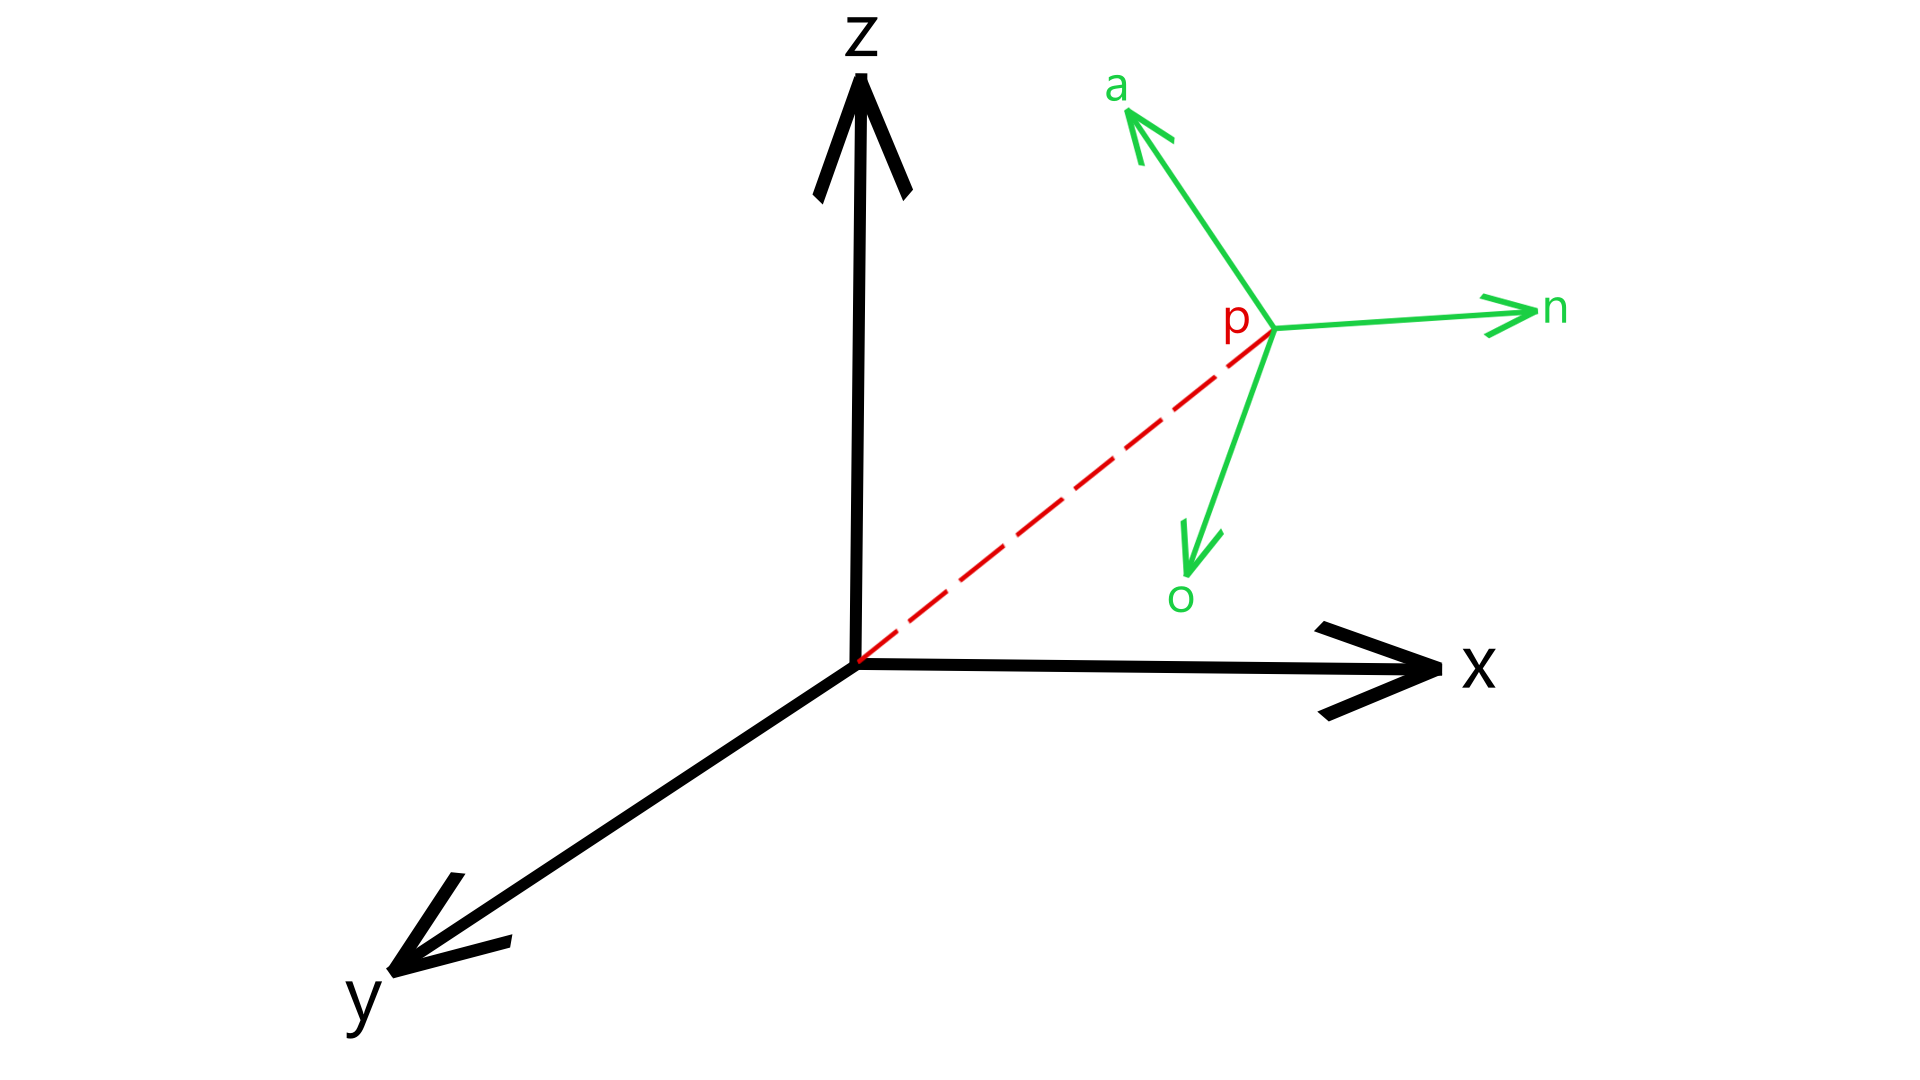
\includegraphics[width=0.7\linewidth]{Sections/2 Problemanalyse/Media/Global og local frames.png}
    \caption{Illustration af global og lokal systemer. De sort akser er det globale system, de grønne akser er et lokal system der tilhøre punktet p. Punktet p repræsenterer et led.}
    \label{fig:Global og lokal systemer}
\end{figure}

Navigation i disse systemer sker ved det der kalds inverse kinematic (IK).
Ved IK anvendes positionen af det sidste/yderste led af en robot, til at fastlægge positioner for de forrige led. Dette kan sammenlignes med en hånd der skal nå en kaffe kop, hvortil albuen og skulderens bevægelser fastlægges ud fra hvor hånden skal ende med at være. Ved IK er det som nævnt det sidste led der dirigerer, dette betyder at banen der bliver fastlagt kommer ud fra hvordan den mindste strækning for det sidste led opnås. For at ændre denne bane kan der i strækningerne mellem to waypoints tilføjes yderligere punkter, som robotten skal gennemløbe. Ved at justere disse tilføjede punkter, kan banen derved justeres efter behov.

% Drivkraft
% Hydraulisk aktuator, pneumatisk aktuator & el-motorer
For at opnå bevægelse langs eller omkring robotters led, anvendes der aktuatorer. Der anvendes primært 3 forskellige typer af aktuatorer, i form af hydrauliske aktuatorer, pneumatiske aktuatorer og elmotorer \parencite{Niku2020IntroductionApplications}.

\textbf{Hydraulisk systemer} gør brug af væsker ikke er kompressible og derved kan overføre kræfter, ved at påvirke væsken med et tryk. Der gælder for hydraulisk systemer at desto større tryk, desto større kraft vil væsken overføre. Forholdet mellem tryk forøgningen og forøgelsen af kraften der overføres, følger et tilnærmelsesvis proportional forhold. Dette betyder at hydrauliske systemer kan udføre opgaver med en god præcision.
 Hydraulisk systemer kan operere med højt tryk, i kombination med deres energitilførselsmekanisme ikke behøver at være monteret på robotarmen, betyder dette at de er velegnet til operationer hvor der skal flyttes tungt gods eller vægten af robotarmen skal være minimal. Hydrauliske systemer har der igennem det bedste energi per vægt forhold, men kræver ofte mere vedligeholdelse end de andre aktuatormuligheder \parencite{Niku2020IntroductionApplications}.

\textbf{Elmotorer} egner sig ligesom hydrauliske systemer godt til præcision, samt kan anskaffes i et bredt spænd af forskellige størrelser og opbygninger \parencite{Kakoty2024IntroductionRobotics}. Dette betyder at elmotorer kan anvendes i et bredt spektrum af opgavestørrelser. I modsætning til hydrauliske systemer, er elmotoren monteret på robot armen og øger derved vægten af armen, som betyder der kræves større kræfter for at sætte armen i bevægelse. 

\textbf{Pneumatisk aktuator} giver minimal præcision da der gøres brug af komprimeret luft, og luft er kompressible, betyder det at der vil være en variation i præcision. Pneumatisk aktuator bruges derfor ofte til led med halve frihedsgrad. Eksempler på brug af pneumatisk aktuator er klemmer der skal løfte og flytte dele \parencite{JHFOSTER2025IdealActuators}. I dette tilfælde er præcision ikke vigtig, da der blots skal trykkes med en givent kraft. Pneumatisk systemer er den type aktuator der kræver mindst vedligeholdelse, grundet en simple opbygning, samt de ikke giver samme anledning til fare for arbejdsulykker ved nedbrud, som de andre hydraulisk aktuator.

Alle tre typer af aktuator kan løse et bredt spænd af opgaver, typen der anvendes vil derfor afhænge af vægtningen af faktorer som pris, præcision, vedligeholdelse og størrelsen af de påkrævede kræfter.